%% -*- coding: utf-8 -*-
\documentclass[12pt,pagesize,paper=192mm:108mm,landscape]{scrbook} 
%1920x1080 1280x720
\areaset[current]{192mm}{108mm}
\usepackage{calc}
\usepackage[T2A]{fontenc}
\usepackage[utf8]{inputenc}
\usepackage[english,russian]{babel}
\usepackage{microtype}
\usepackage{misccorr}
\usepackage{cmap}
%\usepackage[unicode=true]{hyperref}
\usepackage{graphicx}
\usepackage{amssymb}
\usepackage{amsmath}
%\usepackage{srcltx}
\usepackage{textcomp}
\usepackage{xspace}
%научные символы и смайлики \smiley \frownie
\usepackage{wasysym}
\usepackage{ccicons}
\begin{document}
\begin{titlepage}
  \vspace*{-0.5em}
  \begin{center}    
    \hspace*{3em}
    \begin{minipage}[t]{1.5em}
      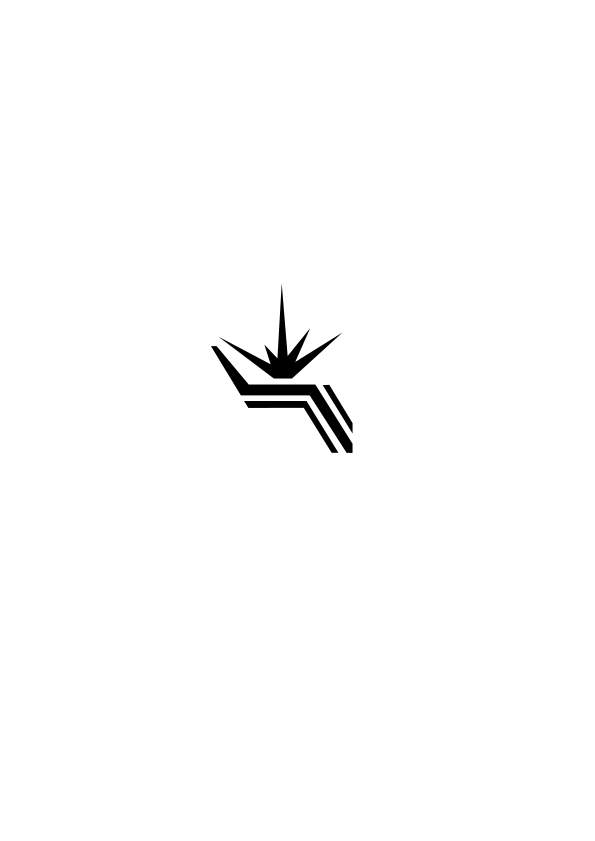
\includegraphics[width=\textwidth]{../BINP-logo}
    \end{minipage}\hfill
    \begin{minipage}{0.115\linewidth}
    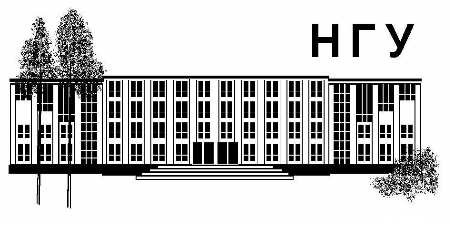
\includegraphics[width=\textwidth]{../NSU-logo}
    \end{minipage}
    \hfill
    \hspace*{4.5em}
    \smallskip

    Кафедра теоретической физики физического факультета НГУ
    \smallskip

    \Large
    Профессор Грабовский А.\,В.

    \huge
    \textbf{Общая теория относительности}
    \smallskip

    \Large
    Лекция № 5
    \vfill

    \normalsize
    \begin{minipage}{0.9\linewidth}
      Гравитационный сдвиг частоты "--- вывод с помощью
      метрики. Приливные силы в Ньютоновском приближении. Уравнение
      расхождения геодезических. Тензор Римана как тензор,
      определяющий приливные силы неустранимые при переходе в
      локально"=геодезическую систему. Отклонение луча света в поле
      солнца: учет искривления пространства за счет $g_{rr}$ и удвоение
      ответа, полученного в первой лекции с помощью принципа
      эквивалентности. Эксперимент Эддингтона, Дайсона и Дэвиса 1919
      года по наблюдению этого отклонения. Уравнение гравитационной
      линзы. Кольцо Эйнштейна. Микролинзирование. MACHO.
     \end{minipage}
    \vfill

    \normalsize \ccbysa\hspace{0.5em}  Новосибирск 2022
  \end{center}
\end{titlepage}
\end{document}
